%************************************************
\chapter{To make a fluorescent tube light circuit}
%************************************************
\begin{flushright}
August 25, 2012
\end{flushright}
\section{Aim}
To make a fluorescent tube light circuit using a ballast.

\section {Tools}
	\begin{enumerate}
		\item Pliers
		\item Screwdriver
		\item Electrical Line Tester
	\end{enumerate}
\section {Material}
	\begin{enumerate}
		\item Tube Light
		\item Tube Light Holder
		\item Electronic Ballast
		\item Bakelite Sheet
		\item Nuts
		\item Bolts
		\item Wires
	\end{enumerate}
\section{Procedure}
	Connected the circuit according to the circuit diagram as given in \autoref{E4_fig1}, keeping the following in mind
	\begin{enumerate}
		\item \emph{Red Wires} are used for the phase connections.
		\item \emph{Black Wires} are used for the neutral connections.
		\item Colours other than Red, Black and Green can be used for the connecting wires.
	\end{enumerate}	
	
	\begin{figure}[bth]
		\begin{center}
			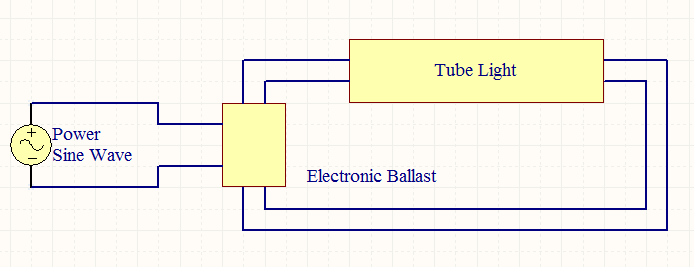
\includegraphics[width=1.2\linewidth]{gfx/circuit4}
		\end{center}
	\caption[Redistribution Board]{Redistribution Board}\label{E4_fig1}
	\end{figure}

\section{Precaution}
	\begin{enumerate}
		\item Connections should be tight, viz. shouldn't come out when pulled.
		\item Wires shouldn't be sticking out of the connections without insulation.
		\item Wires should be of appropriate length.
		\item Colours of the wires should be chosen in accordance with their type.
		\item All tools used must be insulated at their handles.
	\end{enumerate}	
\section{Acknowledgements}
I thank Mr. Jatinder Singh for his guidance during the experiment.